% PREAMBULE
% !BIB TS-program = biber
% !TEX TS-program = xelatexmk
% ITEX TS-program = latex
% !TEX spellcheck = French

\documentclass[class=article, crop=false]{standalone}
\usepackage[subpreambles=true]{standalone}
\usepackage{import}
\usepackage{blindtext}
\usepackage{fontspec}
\usepackage[french]{babel}
\usepackage{caption}
\usepackage{subcaption}
\usepackage{csquotes}
\usepackage{url}

%%%%%%%%%%%%%%%%%%%%%%%%
%			REFERENCES
% le package hyperref avec des options, si en local
\usepackage{hyperref}
\usepackage[backend=bibtex, sorting=nyt, style=verbose-ibid]{biblatex}
\addbibresource{../../../bib.bib}

%%%%%%%%%%%%%%%%%%%%%%%%
%			GLOSSAIRE
\usepackage[acronym]{glossaries}
\makeglossaries
\newglossaryentry{htr}
{
    name=Handwritten Text Recognition,
    description={La reconnaissance du texte écrit sur une image numérique}
}
\newacronym{HTR}{HTR}{Handwritten Text Recognition}

\newglossaryentry{ocr}
{
    name=Optical Character Recognition,
    description={La reconnaissance des polices du texte sur une image numérique}
}
\newacronym{OCR}{OCR}{Optical Character Recognition}

\newglossaryentry{Inria}
{
    name=Inria,
    description={Institut national de recherche en sciences et technologies du numérique}
}
\newacronym{INRIA}{Inria}{Institut national de recherche en sciences et technologies du numérique}

\newglossaryentry{enc}
{
    name=École nationale des chartes,
    description={Grande école bla bla bla}
}
\newacronym{ENC}{ENC}{École nationale des chartes}

\newglossaryentry{HTR-United}
{
    name=HTR-United,
    description={HTR-United is a catalog and an ecosystem for sharing and finding ground truth for optical character or handwritten text recognition (OCR/HTR)}
}

\newglossaryentry{CLab}
{
	name=CREMMALab,
	description={Consortium pour la reconnaissance
d’'écriture manuscrite des matériaux anciens}
}
\newacronym{CREMMA}{CREMMA}{Consortium Reconnaissance
d’Écriture Manuscrite des Matériaux Anciens}

\newglossaryentry{tei}
{
	name={Text Encoding Initiative},
	description={Normes internationales de l'encodage des documents texts}
}
\newacronym{TEI}{TEI}{Text Encoding Initiative}

\newglossaryentry{iiif}
{
	name={International Image Interoperability Framework},
	description={Normes internationales de l'exploitation des images numériques et de leurs métadonnées par API}
}
\newacronym{IIIF}{IIIF}{International Image Interoperability Framework}

\newacronym{ALTO}{ALTO}{Analyzed Layout and Text Object}
\newacronym{XML}{XML}{eXtensible Markup Language}
\newacronym{BNF}{BnF}{Bibliothèque nationale de France}
\newacronym{almanach}{ALMAnaCH}{Automatic Language Modelling and Analysis \& Computational Humanities}
\newacronym{RDF}{RDF}{Resource Description Framework}
\newacronym{TAL}{TAL}{Traitement automatique des langues}


\begin{document}
Le projet \textit{Gallic(orpor)a} s'est développé à partir de plusieurs projets précédents et il tire parti de divers domaines de recherche. Ses créateurs, en mettant en valeur leurs propres connaissances, ont visé à assembler un pipeline qui pourrait traiter les documents issus de la base de données du portail Gallica de la \acrlong{BNF} (\acrshort{BNF}). Les chercheurs spécialisés en \textit{l'\acrlong{HTR}} (\acrshort{HTR}), en \acrlong{TAL} (\acrshort{TAL}), en Histoire, en littérature, mais aussi en lexicographie et en la stylométrie se sont rassemblés pour réaliser ce projet. Le pipeline réalisé dans le cadre du projet \textit{Gallic(orpor)a} a pour but de traiter automatiquement des collections de document aussi bien en ancien-français, moyen français que français classique, issus soit de manuscrits soit d'imprimés produits entre le \textsc{xv}\textsuperscript{e} siècle et le \textsc{xviii}\textsuperscript{e} siècle. Cependant, le but sous-jacent du projet serait de parvenir à produire un prototype qui pourrait servir d'exemple pour mettre en place des chaines d'acquisition numérique pour des collections de documents issus des institutions patrimoniales.

Les ambitions du \textit{Gallic(orpor)a} ont été rendues possibles grâce aux recherches de plusieurs chercheurs et ingénieurs, tels que Laurent Romary, Philippe Gambette, Thibault Clérice, Pedro Suarez Ortiz, Claire Jahan, Caroline Corbières, et Alexandre Bartz. Mais les acteurs principaux du projet \textit{Gallic(orpor)a} lors de mon stage en 2022 étaient Jean-Baptiste Camps, Simon Gabay, et Ariane Pinche, qui ont développé des modèles \acrshort{HTR} pour extraire du texte des documents numériques dans la base de données Gallica. Chez \Gls{Inria}, en tant que stagiaire, j'ai aussi travaillé en collaboration avec Benoît Sagot et Rachel Bawden, qui ont développé des outils d'analyse linguistique. Tous ensemble, ces chercheurs ayant des spécialités diverses ont mis en commun leurs connaissances pour produire un processus du traitement des documents polyvalent.

%%%%%%%%%%%%%%%%%%%%%%%%
%			1. CONTEXTE DU PROJET
\section{Le contexte du projet}

\subsection{Bibliothèque nationale de France et le DataLab}
Le DataLab a été mis en place au sein de la \acrlong{BNF} (\acrshort{BNF}) en 2021\footcite{carlinBnFDataLabService2021}. Lors de sa première année, un premier appel à projets a été lancé  pour mettre en valeur les fonds et les ressources de l'institution phare patrimoniale. Le projet \textit{Gallic(orpor)a} faisait partie des premiers projets acceptés en 2021, à côté des projets \textit{AUREJ} (Accès Unifié aux REssources de la Jouabilité), \textit{GALLICAENV}, \textit{BUZZ-F}, et \textit{AGODA} (Analyse sémantique et Graphes relationnels pour l’Ouverture et l’étude des Débats à l’Assemblée nationale)\footcite[123]{bibliothequenationaledefranceRapportActivite20212022}. Ayant sa candidature retenue, \textit{Gallic(orpora)} a profité d'un financement du DataLab de la \acrshort{BNF}. La plupart du travail sur le projet a eu lieu pendant la première moitié de l'année 2022, grâce à la mise en place de notre stage et de vacations pour la création de données d'entrainement.

\section{Inria et l'équipe ALMAnaCH}
\Gls{Inria} est l'\acrlong{INRIA} et il compte plusieurs branches dans le monde. La branche parisienne accueille l'équipe \acrshort{almanach} dont l'acronyme signifie \textit{\acrlong{almanach}}. Au sein d'\acrshort{almanach} s'est développé le meilleur modèle \acrshort{TAL} pour la langue française, CamemBERT\footcite{martinCamemBERTTastyFrench2020}. L'équipe \acrshort{almanach} encadre des chercheurs, des ingénieurs, des doctorants, et des stagiaires attachés aux projets concernés, soit par le traitement automatique des langues, soit par les humanités numériques. L'acronyme du nom du laboratoire fait référence à ces deux pôles de recherche~: \textit{Automatic Language Modelling and Analysis} est le traitement automatique des langues, et  \textit{Computational Humanities} pour les humanités numériques. Le projet \textit{Gallic(orpor)a} se situait entre les deux, impliquant l'extraction des données et l'édition des documents historiques, ainsi que l'analyse linguistique du texte extrait.

Benoît Sagot, directeur de recherches d'\acrshort{almanach}, s'est chargé de l'encadrement du stage du projet \textit{Gallic(orpor)a}. En tant que stagiaire, je faisais partie de l'équipe de début avril et à fin juillet 2022. Pendant le stage, Rachel Bawden a animé un groupe de lecture hebdomadaire et des séminaires mensuels sur les nouvelles recherches et les nouveaux enjeux en le \acrlong{TAL}. Elle a aussi développé un modèle \acrshort{TAL} pour le projet \textit{Gallic(orpor)a} et m'a guidée dans sa mise en œuvre\footcite{bawdenAutomaticNormalisationEarly2022, gabayFreEMcorporaFreEMnormFreEM2022}. J'ai travaillé en présentiel quatre jours par semaine, en passant un jour toutes les semaines à l'\Gls{enc} pour travailler à côté de l'une des chefs du projet, Ariane Pinche. Chez \Gls{Inria}, j'ai profité de l'expertise de mes collègues de l'équipe \acrshort{almanach}, en particulier d'Alix Chagué et d'Hugo Scheithauer. L'équipe entière de \textit{Gallic(orpor)a} a aussi profité des serveurs d'\Gls{Inria}, qui prenaient en charge une partie de la puissance de calcul et du stockage de données pour l'interface graphique \acrshort{HTR} \textit{eScriptorium}.

\subsection{École nationale des chartes et l'université de Genève}

Ariane Pinche, post-doctorante à l'\acrlong{ENC}, et Simon Gabay, maître-assistant à l'université de Genève,  ont géré la mise en place du stage et des vacations que la bourse du Data Lab de la \acrshort{BNF} a permis de financer. Deux autres chercheurs qui étaient attachés à l'\acrlong{ENC} pendant le stage, Jean-Baptiste Camps et Thibault Clérice, ont également contribué au projet \textit{Gallic(orpor)a}. S. Gabay et A. Pinche se sont occupés de l'harmonisation des vérités de terrain produites par l'équipe en relisant toutes les transcriptions que les vacataires ont faites dans l'interface graphique \textit{eScriptorium}. A. Pinche et T. Clérice ont commencé à utiliser les vérités de terrain des documents médiévaux en entraînant de nouveaux modèles  \acrshort{HTR} et de segmentation\footcite{clericeYALTAiSegmontoManuscript2022}. Pour la segmentation, J.-B. Camps, A. Pinche, et S. Gabay ont développé la syntaxe \textit{SegmOnto} qui sert à harmoniser les vérités de terrain produites du corpus d'entraînement\footcite{gabaySegmOntoCommonVocabulary2021}. Bien que chaque chercheur ait ses spécialités, ils ont tous collaboré et le projet a pu profiter des expertises de chacun.

\section{La création des données d'entrainement du projet}
\label{veritesDeTerrain}
Le projet \textit{Gallic(orpor)a} vise à développer et mettre en place des modèles \acrshort{HTR} pouvant traiter tout document français dans la base de données Gallica créée entre le \textsc{xv}\textsuperscript{e} siècle et la Révolution française. Un corpus de documents sources numérisés ainsi qu'une sélection de leurs pages à transcrire a permis de générer des données d'entraînement. Les documents qui composent ce corpus sont détaillés dans la section \ref{data:portee} de l'appendice. La sélection a été guidée par la volonté d'avoir une certaine diversité de documents, de genre et d'origine géographique. Comme montre la Figure \ref{fig:diversite_genre}, il y avait les manuscrits, les incunables, et les imprimés. De plus, chaque type de document possède des représentants issus de plusieurs genres littéraires: poésie, récit, et le traité. Dans le cas des imprimés, il y avait aussi des pièces de théâtre.

\begin{figure}[hbt!]
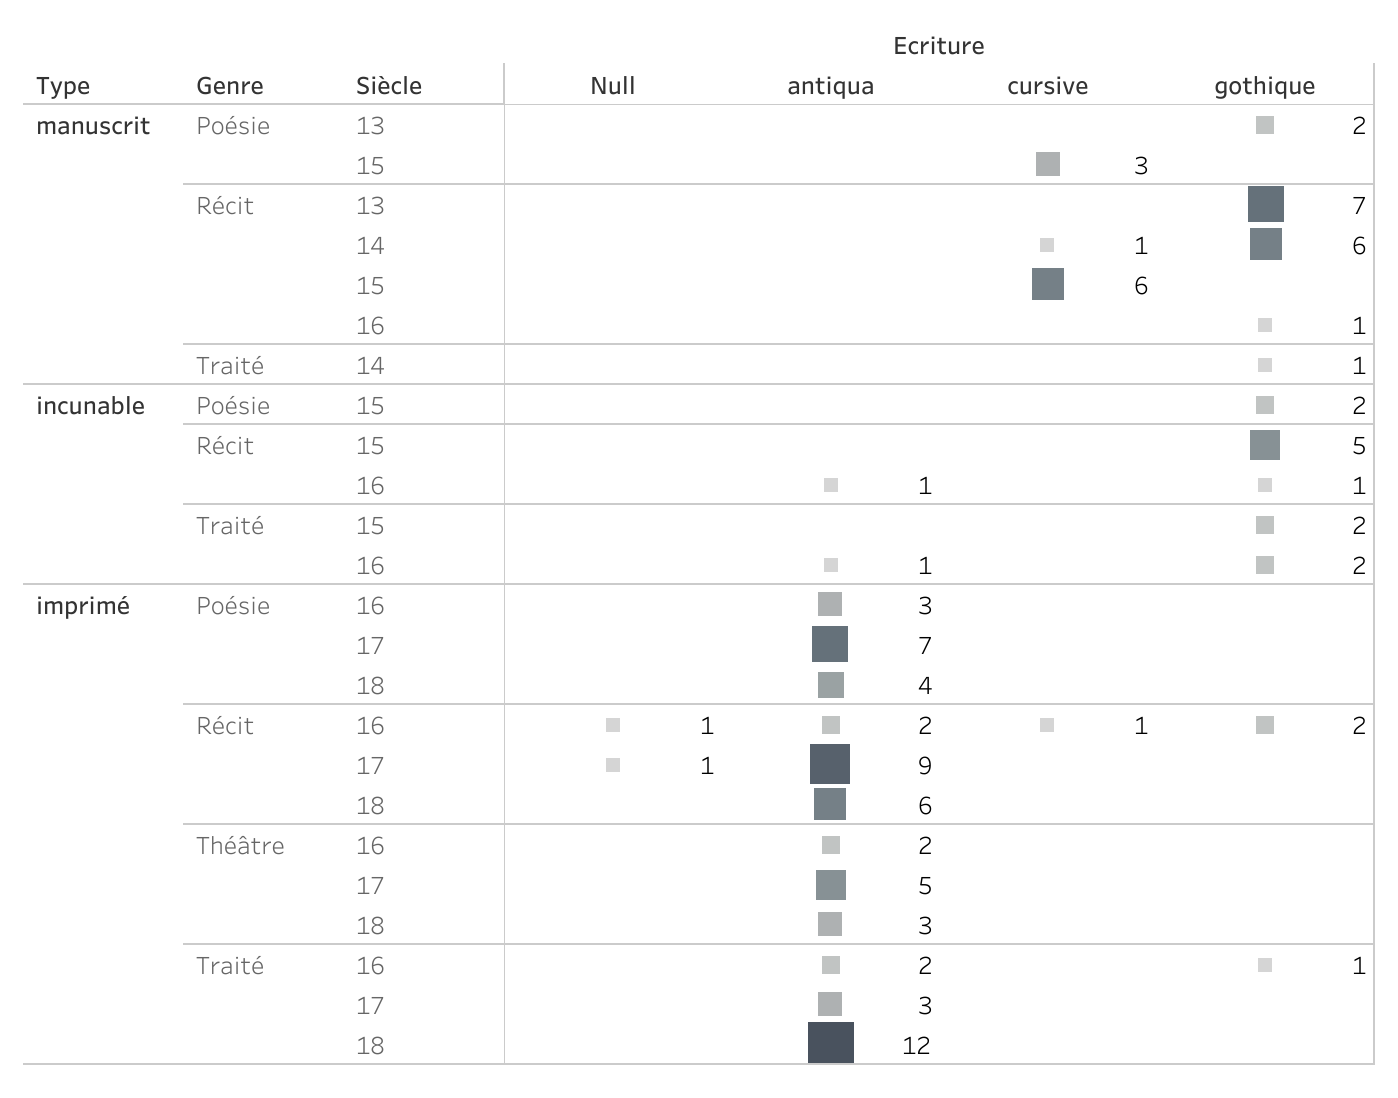
\includegraphics[width=\textwidth]{../../../images/diversite_genre.png}
\caption{Diversité documentaire et générique}
\label{fig:diversite_genre}
\end{figure} 
% attention tu as mis diversité linguistique pour documentaire antiqua, cursive et gothique sont des types de police ou d'écriture.

Pour terminer, un autre souhait quant à la diversité du corpus a porté sur le lieu de publication ou d'apparition du document, comme montre la Figure \ref{fig:diversite_ville}. La plupart des documents choisis de la base de données Gallica étaient issus de Paris, à l'image de la collection de la Bibliothèque nationale de France. Toutefois, une partie importante est également originaire de Lyon. Enfin, ont également été inclus des manuscrits, des incunables, et des imprimés écrits en français, venus de villes telles que Londres, Amsterdam, ou encore Rome.

\begin{figure}[hbt!]
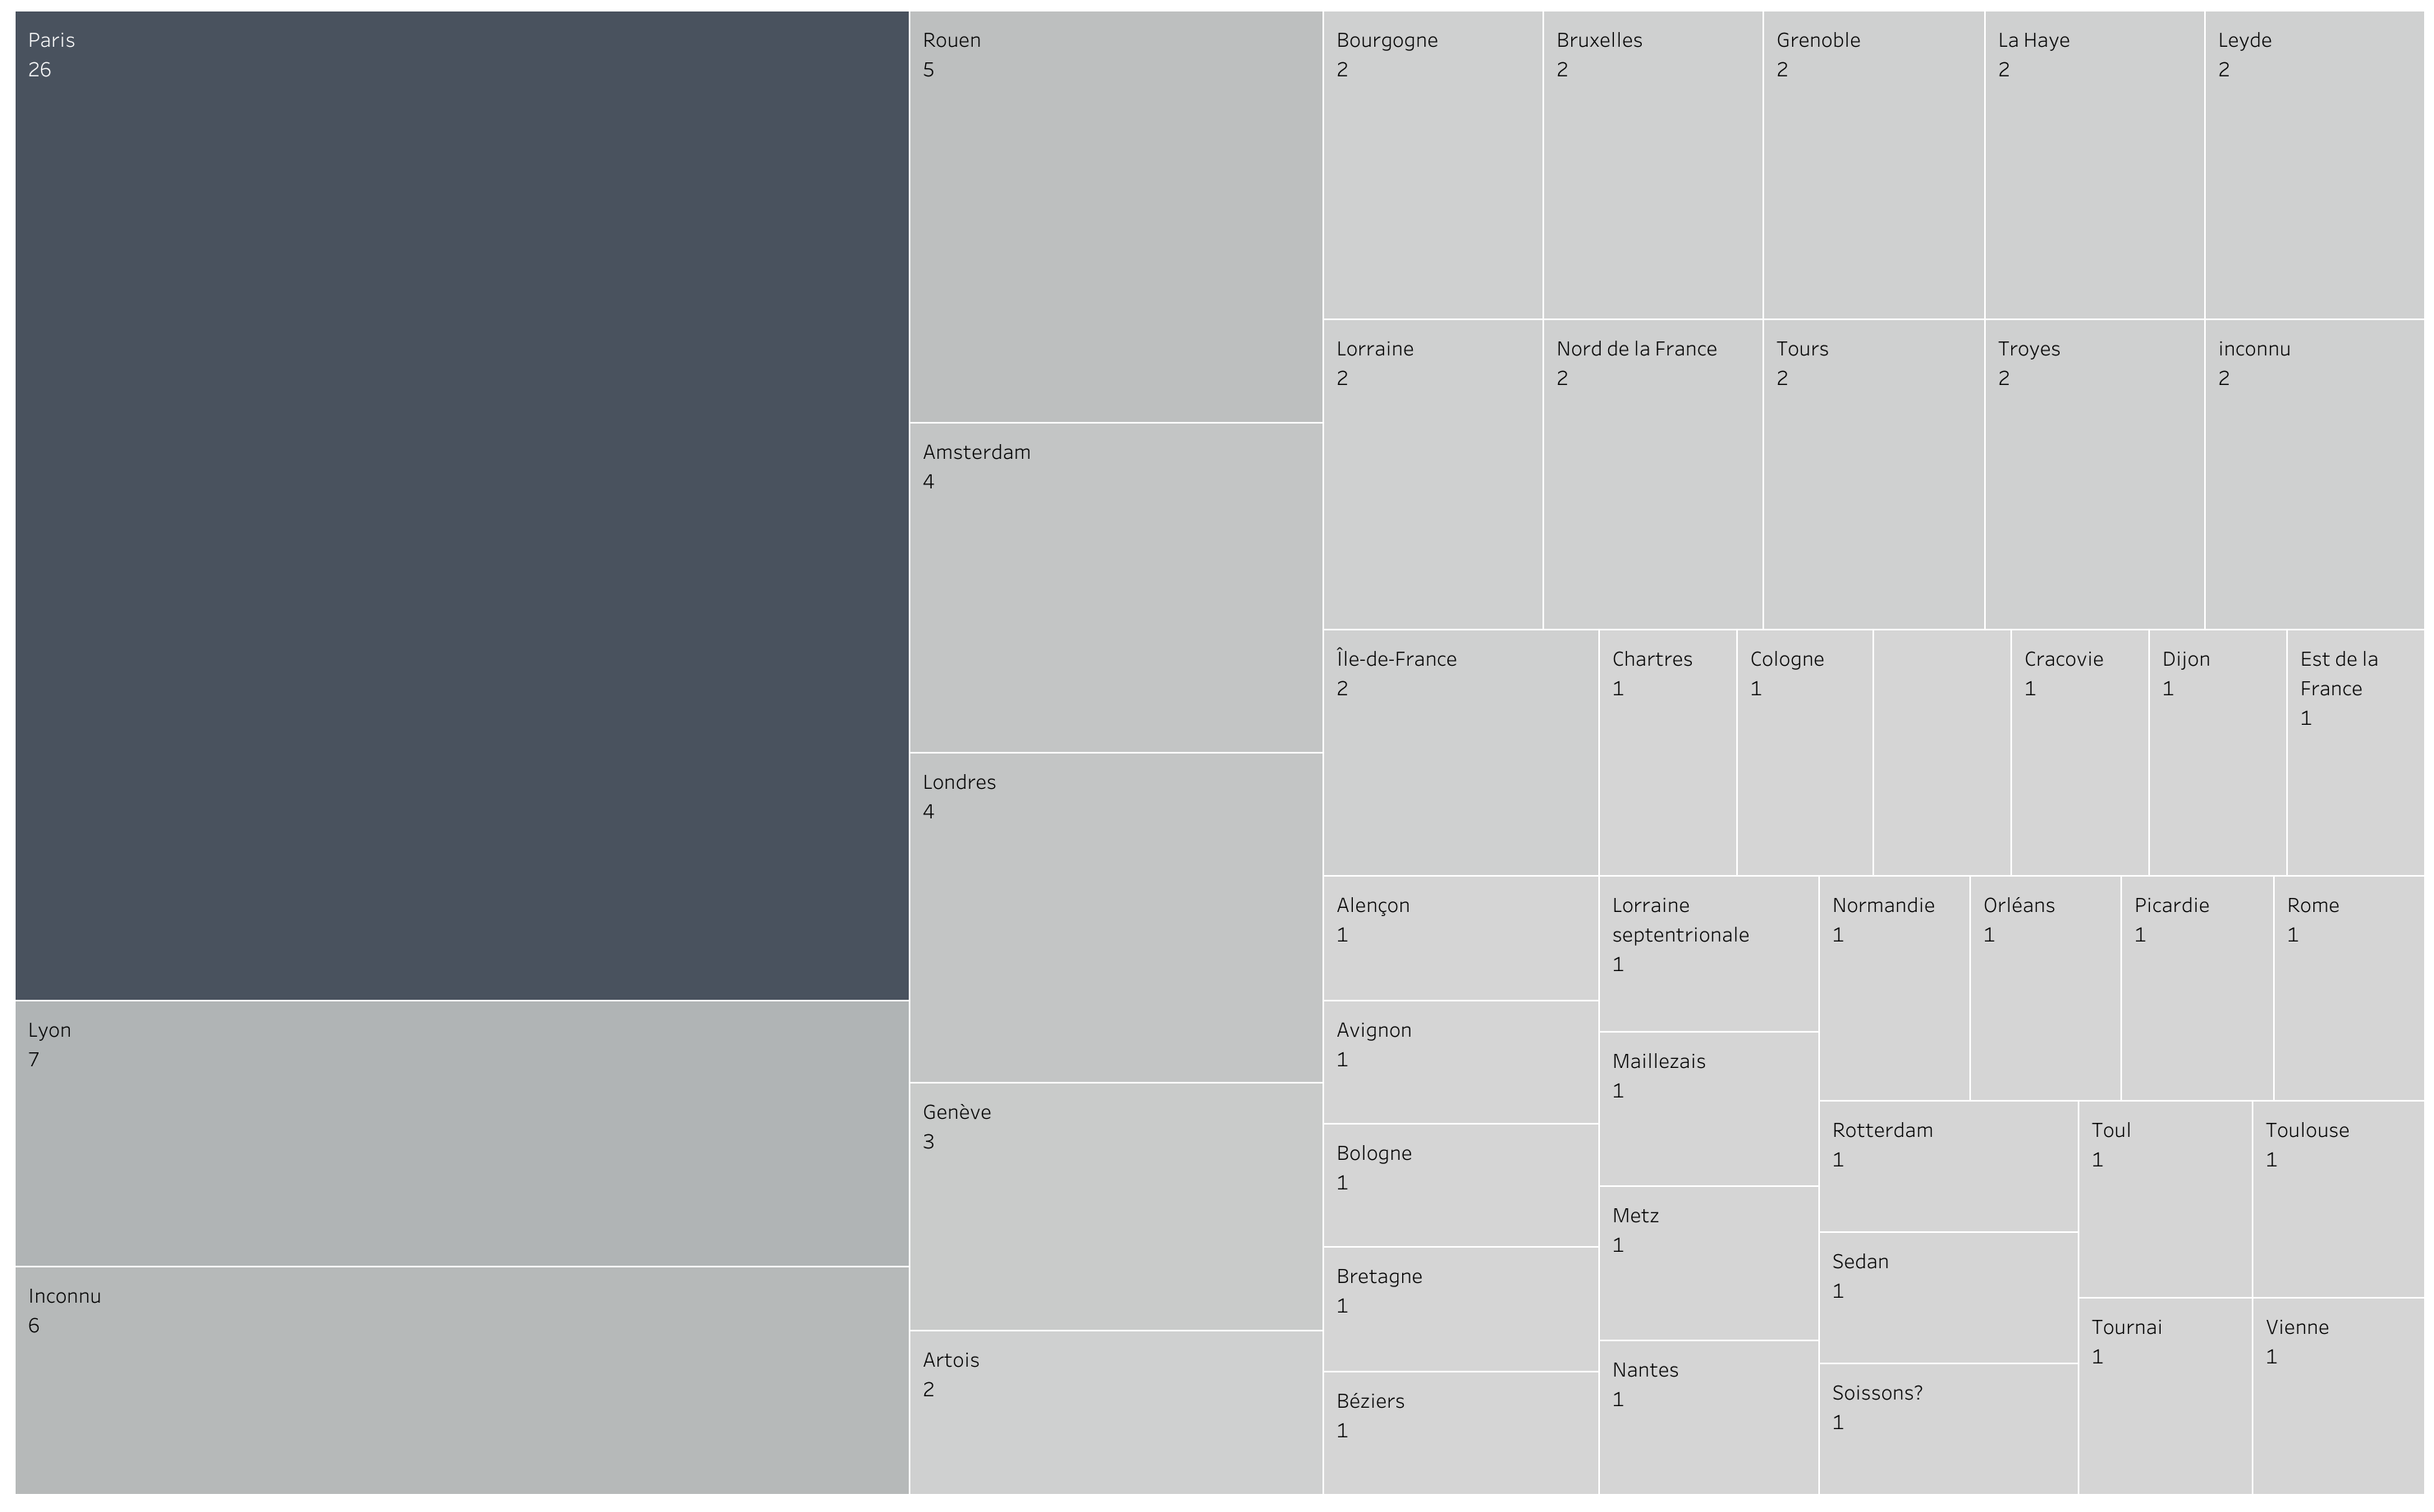
\includegraphics[width=\textwidth]{../../../images/diversite_ville.png}
\caption{Diversité géographique}
\label{fig:diversite_ville}
\end{figure}

Après avoir établi le corpus, les pages ciblées dans chaque document ont été transcrites par des vacataires en utilisant l'interface graphique \textit{eScriptorium}, qui permet à la fois la transcription du texte et la segmentation de la page. La segmentation de la page se fait en mettant les étiquettes précises sur les lignes et les blocs de texte~; ces étiquettes suivent le vocabulaire \textit{SegmOnto}. Ensuite, les vérités de terrain produites avec l'interface graphique \textit{eScriptorium} sont transférées vers les dépôts Github du projet, organisés par siècle et type de document. L'outil \texttt{HTRVX} du projet \Gls{HTR-United} a permis d'analyser toutes les transcriptions transférées pour signaler les erreurs potentielles de segmentation, et ainsi faciliter le nettoyage des données.


\section{Les prédécesseurs du projet}
Comme expliqué avant, \textit{Gallic(orpor)a} a rassemblé les recherches de plusieurs projets précédents. Il a profité des glossaires codicologiques, des progrès dans la prédiction et la segmentation des documents, des progrès dans l'analyse linguistique, et des catalogues des données. Par exemple, le vocabulaire \textit{SegmOnto} permet d'harmoniser les vérités de terrain pour les manuscrits et les imprimés. Les modèles \acrshort{HTR} sont à la fois l'un des livrables du projet et un support pour la production des vérités de terrain, en opérant une transcription préliminaire qui sert à entraîner des nouveaux modèles. En outre, grâce au catalogue Open Source \Gls{HTR-United}, un portail qui agrège des recherches et permet de retrouver des données, les vérités de terrain du projet \textit{Gallic(orpor)a} seront visibles et aisées à retrouver pour d'autres projets\footcite{chagueSharingHTRDatasets2022}. Enfin, l'analyse linguistique est également un objectif du projet \textit{Gallic(orpor)a}, et la mise en œuvre de cet aspect s'appuie sur les modèles de la langue française construits par les chercheurs de l'équipe \acrshort{almanach}. Toutefois, ce point n'a pas encore été ajouté au pipeline du projet.


\subsection{Le glossaire codicologique}
Le projet \textit{Gallic(orpro)a} a produit des données en accord avec le vocabulaire \textit{SegmOnto}, qui est expliqué en détail dans le chapitre \ref{chap:segmonto}. Ayant géré les données produites selon cette codicologie, j'ai aussi contribué à l'élaboration et le perfectionnement du vocabulaire. La décision d'utiliser la syntaxe descriptive des lignes et des zones de \textit{SegmOnto} a été prise dès la mise en œuvre du projet \textit{Gallic(orpor)a}. La généricité du vocabulaire permet de traiter des documents très divers dans le cadre du projet. Comme \textit{Gallic(orpor)a} vise à livrer un prototype d'un pipeline qui pourrait traiter tout document source numérisé, la généralisation des étiquettes appliquées aux lignes et aux zones était impérative, et le vocabulaire de \textit{SegmOnto} la meilleure solution.

\subsection{La segmentation et la prédiction du texte}
Les progrès de la reconnaissance du texte sont expliqués en détail dans le chapitre \ref{chap:htr}. Un logiciel \acrshort{HTR} commence par la segmentation de la page, et dès qu'il sait où se trouvent les caractères, les mots, et les lignes du texte, il le prédit à partir de l'écriture. Ces deux tâches se font selon les compétences qu'il a apprises lors de son entraînement. Dans le but de produire les vérités de terrain pouvant entraîner les modèles \acrshort{HTR} pour les manuscrits, les incunables, et les imprimés dans la base de données Gallica, le projet \textit{Gallic(orpor)a} a profité de l'expertise de Simon Gabay et d'Ariane Pinche, qui s'occupaient de la relecture des vérités de terrain et la gestion des corpus d'or.

Les progrès dans la prédiction du texte sur les imprimés de l'Ancien Régime ainsi que son analyse ont aidé le projet \textit{Gallic(orpor)a}. Par les imprimés françaises de l'Ancien Régime, S. Gabay a entraîné les modèles sur les vérités de terrain des imprimés du \textsc{xvi}\textsuperscript{e} au \textsc{xviii}\textsuperscript{e} siècle\footcite{gabayStandardizingLinguisticData2020}. En collaboration avec d'autres chercheurs, il a travaillé sur le jeu de données OCR17+ qui a fourni des vérités de terrain des imprimés du \textsc{xvii}\textsuperscript{e} siècle\footcite{gabayOCR17GroundTruth2020}. Pour tester le pipeline, dans l'attente des modèles nouvellement entraînés sur les données produites dans le cadre de \textit{Gallic(orpor)a}, j'ai utilisé un modèle de segmentation et un modèle d'\acrshort{HTR} que Gabay a développé dans le cadre de son projet \textit{E-ditiones}\footcite{gabayEditiones17thFrench2018}.

Pour la reconnaissance du texte sur les documents médiévaux, le projet \Gls{CLab} est la clef. Géré dans le cadre des études postdoctorales d'Ariane Pinche, le \acrlong{CREMMA}, ou \acrshort{CREMMA}, est un dépôt des images et leurs transcriptions corrigées à la main, soit des vérités de terrain. Afin d'entraîner un modèle \acrshort{HTR}, il faut un jeu des vérités de terrain\footcite{chagueHTRUnitedMutualisonsVerite2021}. Le projet \Gls{CLab} fournit un jeu des vérités de terrain de 13 manuscrits médiévaux qui se composent de 21~656 lignes de texte transcrites\footcite{pincheCremmaLabProjectTranscription2022}. Sur les données du projet, A. Pinche a entraîné un modèle \acrshort{HTR} qui est désormais disponible sur Zenodo\footcite{pincheHTRModelCremma2022}. Le projet \textit{Gallic(orpor)a} en a également permis la création de vérités de terrain pour les manuscrits médiévaux.

\subsection{Harmonisation et partage des données}
Le projet \Gls{HTR-United} permet de cataloguer des vérités de terrain générées par tout projet \textit{open source}\footcite{chagueHTRUnitedHtrunitedV02022}. Sa base de données, librement mise en ligne par GitHub, contient les images et leurs transcriptions faites par plusieurs projets de recherche. Elle comporte sur les documents de plusieurs périodes historiques et écritures. Un modèle \acrshort{HTR} peut être entraîné sur ces jeux de données. Par exemple, Alix Chagué a entraîné un modèle \acrshort{HTR} sur les vérités de terrain du \textit{LECTAUREP Project}, soutenu par \Gls{Inria} et les Archives Nationales, qui sont recensées sur la base de données \Gls{HTR-United}\footcite{chagueLECTAUREPContemporaryFrench2022}.

Dans l'esprit de la science ouverte, toutes les vérités de terrain produites par le projet \textit{Gallicorpora} apparaissent dans le catalogue \Gls{HTR-United}. À la fin du stage, en juillet 2022, Ariane Pinche et Thibault Clérice ont entraîné un modèle pour les manuscrits médiévaux en utilisant les transcriptions que l'équipe du projet \textit{Gallic(orpor)a} a produites. Ces vérités de terrain sont désormais mises en commun sur \Gls{HTR-United} et A. Pinche et T. Clérice ont lié le premier modèle publié du projet \textit{Gallic(orpor)a} avec le catalogue \Gls{HTR-United} et le dépôt du projet \acrshort{CREMMA} (\acrlong{CREMMA})\footcite{pincheHTRUnitedCremmamedievalCortado2022}. Le partage des données du projet est l'un de ses objectifs.

\subsection{L'analyse linguistique}
Après l'extraction et le nettoyage des données des documents source de Gallica, le projet \textit{Gallic(orpor)a} a envisagé de lemmatiser les textes. Dans cet objectif, il a profité des derniers progrès dans le domaine de l'analyse linguistique du français classique. L'analyse linguistique du français de l'Ancien Régime, tel que ce qui se voit dans les écrits de Molière, est un domaine de recherche actuellement en plein développement. Depuis une dizaine d'années, les chercheurs en linguistique computationnelle ont élaboré des outils pour analyser des états de langue ancien du français. La recherche dans le domaine du français contemporaine quant à elle est déjà bien ayant bénéficié de jeux de données plus nombreuses et accessibles et de financements privés liés à ces applications commerciales.

L'histoire de l'analyse linguistique et du \acrlong{TAL} (\acrshort{TAL}) est trop riche pour être retracée ici. Néanmoins, quelques étapes méritent d'être rappelées. Achim Stein a abordé le sujet de l'analyse linguistique du français du Moyen Âge dans son article de 2013\footcite{steinSyntacticAnnotationMedieval2013}. Dans le même année, il a collaboré avec Sophie Prévost pour créer un \textit{treebank} pour l'ancien français, le \textit{Syntactic Reference Corpus of Medieval French} (SRCMF)\footcite{steinSyntacticReferenceCorpus2013}. En 2014, Prévost est des autres chercheurs, Gael Guibon, Isabelle Tellier, Matthieu Constant, et Kim Gerdes, ont soutenu que la variation de lexique de l'ancien français pose un défi à l'analyse linguistique\footcite{guibonParsingPoorlyStandardized2014}. En 2019, Mathilde Regnault, S. Prévost, et Éric Villemonte de La Clergerie ont utilisé le SRCMF avec le MCVF (Modéliser le changement : les voies du français) pour mieux décrire et structurer notre connaissance de l'évolution du français\footcite{regnaultChallengesLanguageChange2019}. Ces études ont été des pionnières qui nous permettent aujourd'hui de mieux élaborer des modèles pour analyser des textes historiques en ancien français. Un exemple d'une telle élaboration récente est le modèle \textit{Deucalion}. Jean-Baptiste Camps, Simon Gabay, Paul Fièvre, Thibault Clérice, et Florian Cafiero l'ont créé pour le français de l'Ancien Régime, en l'entraînant sur les livrets des drames du \textsc{xvii}\textsuperscript{e} siècle\footcite{campsCorpusModelsLemmatisation2021}. Le développement des nouveaux modèles TAL pour les anciens états du français a rendu possible la mise en œuvre éventuelle d'une telle étape d'analyse au pipeline de \textit{Gallic(orpro)a}.


%%%%%%%%%%%%%%%%%%%%%%%%
%			3. PIPELINE
\section{Le pipeline}
Outre la création des vérités de terrain, qui est expliqué dans une section précédente (Section \ref{veritesDeTerrain}), le projet \textit{Gallic(orpor)a} vise à pouvoir générer une ressource numérique qui porte sur le document source en liant une transcription des pages avec deux versions du texte, l'une pré-éditorialisée et l'autre soumise à l'analyse linguistique. En commençant par les pages numérisées du document source, la ressource numérique présente quatre types d'information~:
\begin{enumerate}
\item les métadonnées à propos du document source
\item la transcription du document, prédite par les modèles \acrshort{HTR}
\item le texte pré-éditorialisé du document source
\item le texte analysé par les outils \acrlong{TAL} (\acrshort{TAL})
\end{enumerate}


Chaque type d'information offre un panel de possibilité dans l'usage des données textuelles. Les métadonnées s'informent sur trois types de document concerné par le pipeline~: (1) la ressource numérique qu'il créé, (2) le fac-similé numérique du document source d'où vient la transcription par \acrshort{HTR}, (3) le document source physique qui se conserve quelque part, sinon qui a été conservé avant sa disparition, et qui est à l'origine du fac-similé numérique. Les données produites par les modèles \acrshort{HTR} contiennent la segmentation de la mise en page et la prédiction du texte. Ensuite, le texte pré-éditorialisé est présenté, sans sa segmentation, d'une manière plus propice à l'analyse linguistique. Et enfin, le fichier final devrait proposer une analyse linguistique du texte grâce à l'application de certains modèles \acrshort{TAL}.

Voir la représentation du pipeline sur la Figure~\ref{fig:pipeline}. En bleu les saisies des données, en vert les fichiers préliminaires que le pipeline construit, en orange sa première sortie, et en violet les divers moyens d'exploitation de sa sortie. Comme le pipeline permet de générer des métadonnées et la transcription, il a besoin d'au moins deux saisies des données. L'une porte sur les métadonnées des trois types de document concernés (la ressource numérique produite par le pipeline, le fac-similé numérique du document source, le document source physique). Elle se composer de plusieurs sources de données en ligne, afin de fournir à la ressource numérique autant de détail que possible. L'autre saisie des données est l'image numérique elle-même en format JPEG, TIFF, ou PNG.

\begin{figure}[hbt!]
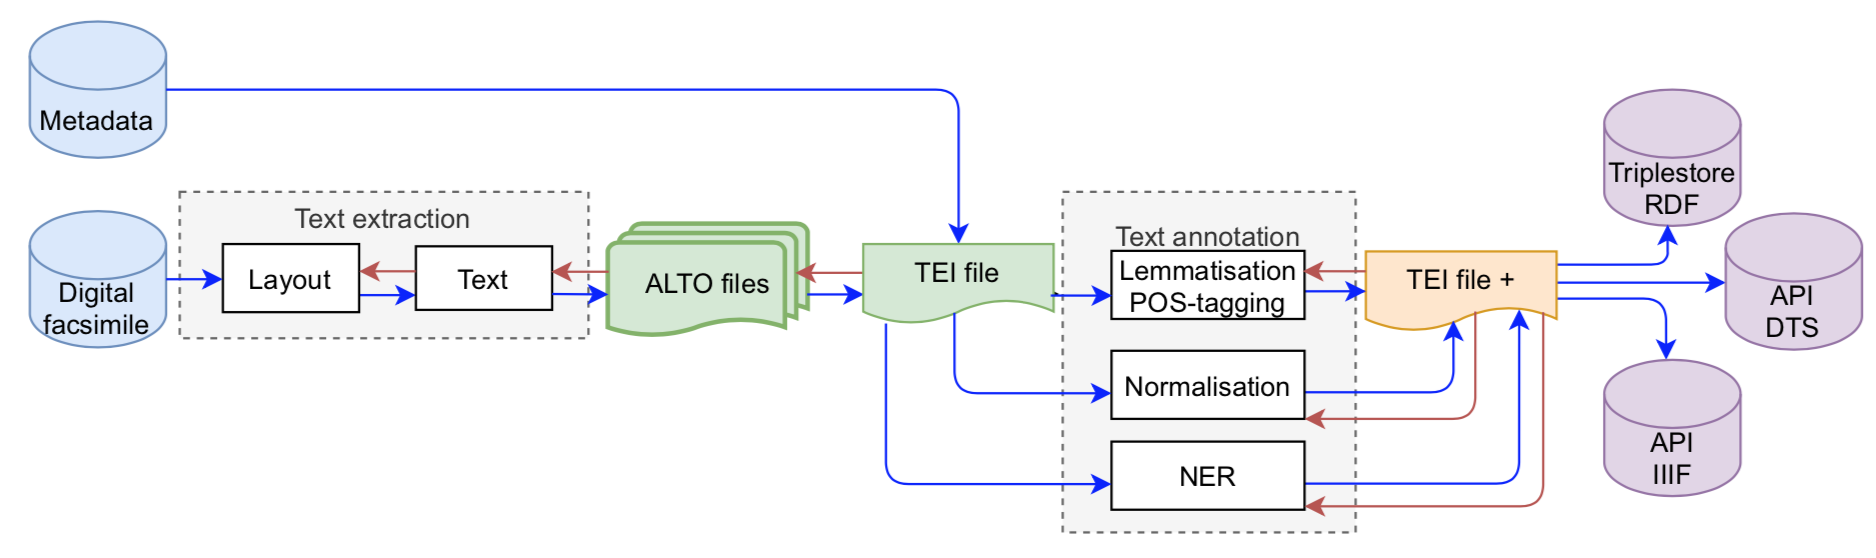
\includegraphics[width=\textwidth]{../../../images/pipeline.png}
\caption{Pipeline}
\label{fig:pipeline}
\end{figure}

La Figure~\ref{fig:pipeline} montre en vert les premiers fichiers préliminaires du pipeline, les fichiers \acrshort{ALTO} et la version du fichier \acrshort{TEI} sans l'analyse linguistique. Les fichiers \acrshort{ALTO} sont d'un format \acrshort{XML} qui ont un schéma particulièrement adapté à l'encodage de l'analyse de la mise en page que fait un modèle de segmentation ainsi qu'à la prédiction du texte que fait un modèle \acrshort{HTR}. Le chapitre~\ref{chap:xml} du mémoire en parle en plus de détail. Son acronyme veut dire en anglais \textit{l'\acrlong{ALTO}}, ou la mise en page analysée et l'objet de texte. Comme le montre la nature bipartite du nom \textit{\acrlong{ALTO}}, les fichiers \acrshort{ALTO} alignent la mise en page et le texte prédit. Le pipeline a créé  ces fichiers en appliquant les modèles \acrshort{HTR} aux données d'entrée visuelles.

Après la création des fichiers préliminaires, le pipeline crée la première version du fichier \acrshort{TEI}, qu'il va plus tard enrichir avec l'analyse linguistique du texte prédit. Ce premier fichier \acrshort{TEI} occasionne la création des métadonnées. Comme le montre la flèche bleue dans la Figure~\ref{fig:pipeline}, les métadonnées sont récupérées depuis les sources en ligne et ensuite nettoyées et intégrées au fichier \acrshort{TEI}. Le fichier \acrshort{TEI} préliminaire récupère aussi les données des fichiers \acrshort{ALTO}.

À la suite de la récupération, du nettoyage, et enfin de la transformation des données des divers sources, le pipeline continue à traiter le texte qu'il a récupéré des fichiers \acrshort{ALTO}. Dans un premier temps, il parse les données récupérées des fichiers \acrshort{ALTO} et extrait toute ligne de texte imbriquée dans une zone qui fait partie du texte principal. Cela veut dire qu'il n'extrait pas de numéro de page, d'en-tête, etc. Les lignes de texte ainsi sélectionnées sont présentées comme le texte pré-éditorialisé du document source. Elles représentent une première transcription du texte, en ignorant la mise en page sauf les sauts de ligne.

Ce texte pré-éditorialisé peut aisément servir à l'analyse qu'une utilisatrice ou un utilisateur voudrait faire en s'appuyant sur le texte tel qu'il apparaît dans le document source. Ce texte sert aussi à la génération d'un texte annoté, issue de l'analyse linguistique des outils \acrshort{TAL}. Le résultat de ce dernier traitement est visualisé dans la Figure~\ref{fig:pipeline} en orange sous le nom de fichier \acrshort{TEI} enrichi, \textit{TEI file +}. Pour terminer, les données de la sortie peuvent être exploitées dans plusieurs formats, comme le montrent les étapes signalées en violet dans la Figure~\ref{fig:pipeline}.

\end{document}
\documentclass[../main.tex]{subfiles}